\documentclass{beamer}

%%%%%%%%%%%%%Solarized Theme%%%%%%%%%%%%%%%
\usecolortheme[light,accent=cyan]{solarized}
\beamertemplatenavigationsymbolsempty
%%%%%Packages%%%%%
\usefonttheme{serif}
\usepackage[T1]{fontenc}
\usepackage[utf8]{inputenc}
\usepackage[english]{babel}
\usepackage{fontawesome}
\usepackage{minted}
\usepackage{soul}
\usepackage{ulem}
\usepackage{blkarray}
\usepackage{multirow}

\definecolor{DarkGray}{gray}{0.1}
\usemintedstyle{paraiso-dark}


\usepackage{graphicx}
\usepackage{hyperref}
\usepackage{colortbl, xcolor}
\usepackage{booktabs}
\usepackage{amsmath,amsthm, amssymb, latexsym}

\usepackage{tikz}
\usepackage{xcolor}
\usepackage{graphicx,multirow}
\definecolor{plain}{rgb}{93,93,93}
\usetikzlibrary{positioning,arrows}
\definecolor{applegreen}{rgb}{0.55, 0.71, 0.0}
\usetikzlibrary{decorations.pathreplacing, backgrounds, fit,}
\usetikzlibrary{calc,matrix}

\tikzstyle{background}=[solarizedRed, rectangle, draw, inner sep=1mm, thick,
           rounded corners=2mm]

\tikzset{
  treenode/.style = {align=center, inner sep=0pt, text centered,
    font=\sffamily},
  arn_n/.style = {treenode, circle, white, font=\sffamily\bfseries, draw=black, inner sep=-6pt,
    fill=black, text width=1.5em},% arbre rouge noir, noeud noir
  arn_r/.style = {treenode, circle, red, 
    text width=1.5em, very thick, inner sep=4pt},% arbre rouge noir, noeud rouge
  arn_x/.style = {treenode, rectangle, draw=black,
    minimum width=0.5em, minimum height=0.5em}% arbre rouge noir, nil
}
\newtheorem{conjecture}[theorem]{Conjecture}
\def\checkmark{\tikz\fill[scale=0.4](0,.35) -- (.25,0) -- (1,.7) -- (.25,.15) -- cycle;} 

\usepackage{standalone}
\usepackage{siunitx}

\newsavebox\MBox
\newcommand\Cline[2][red]{{\sbox\MBox{$#2$}%
  \rlap{\usebox\MBox}\color{#1}\rule[-1.5\dp\MBox]{\wd\MBox}{1.5pt}}}

\begin{document}

\begin{frame}
    \begin{center}
        \textbf{\LARGE{\textcolor{orange}{Good strategies with $n-$bit memory}}} \\
        \vspace{1cm}

        \textbf{@nikoletaglyn}\\
        \vspace{2cm}
        \pause

        \textbf{Christian Hilbe  \; Martin Nowak \; Ethan Akin}
    \end{center}
\end{frame}

\begin{frame}
    \begin{center}
    \begin{columns}
        \begin{column}{.6\textwidth}
            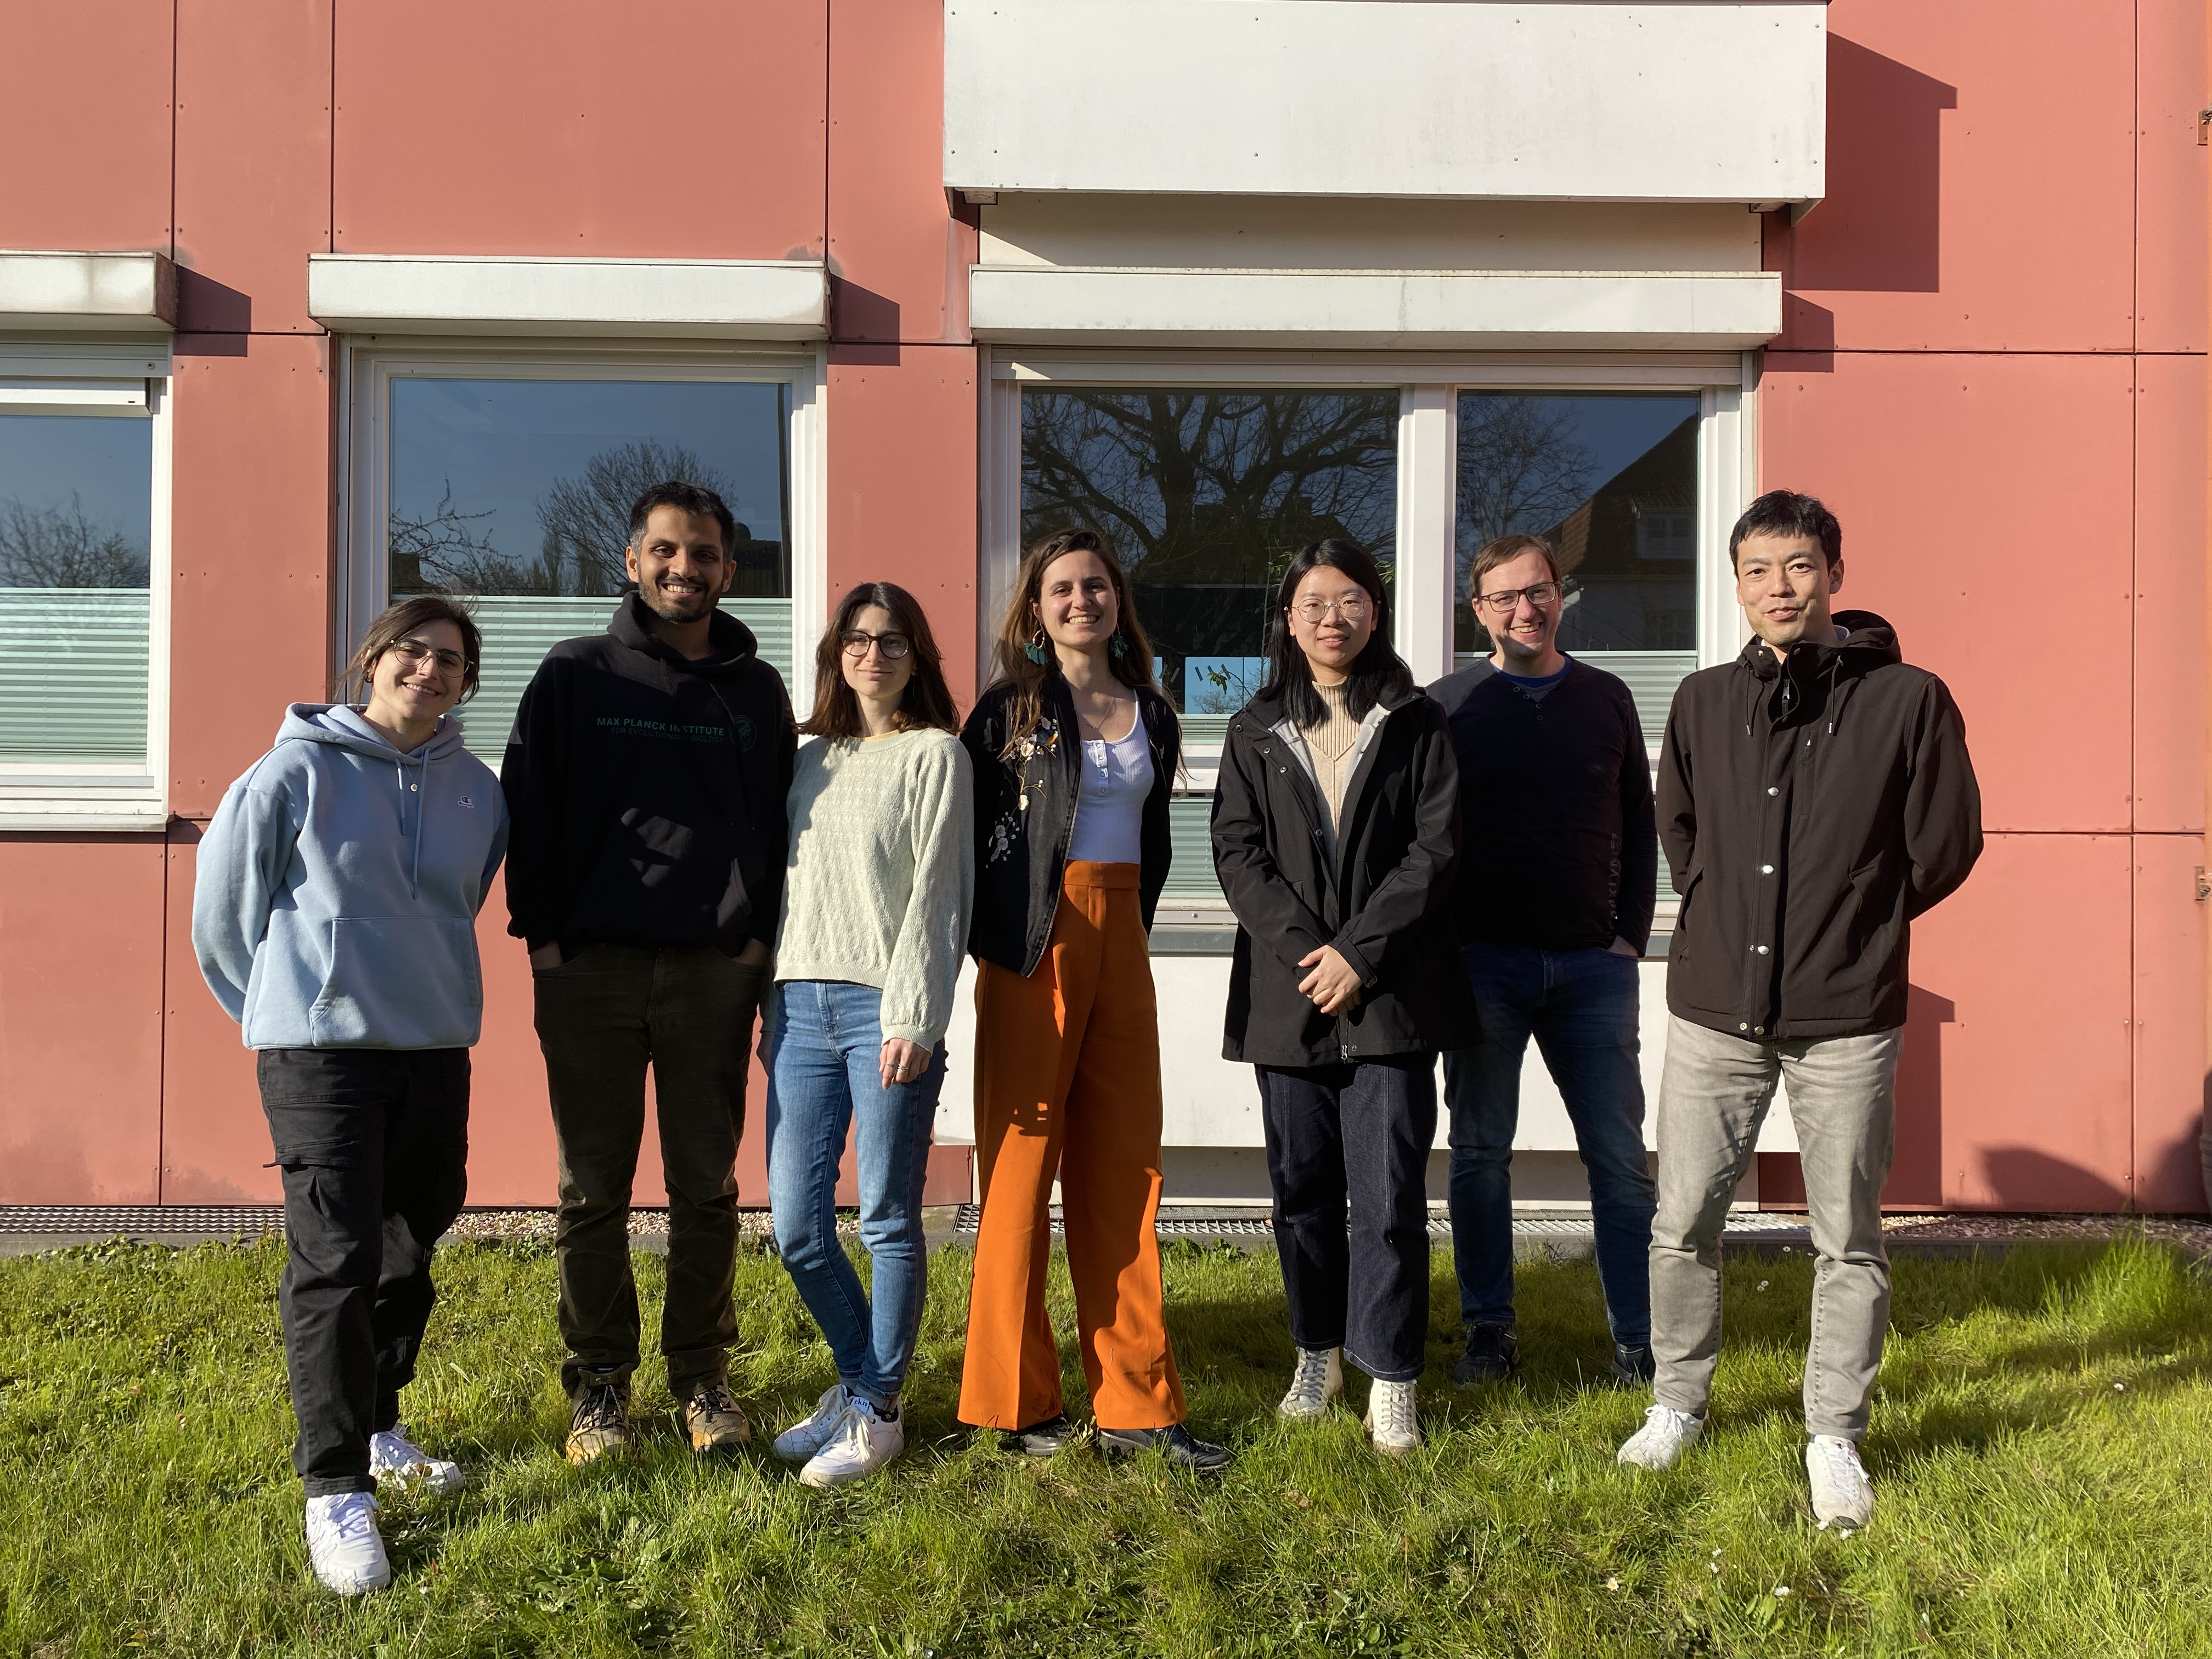
\includegraphics[width=\textwidth]{static/group.jpg}
        \end{column}
        \begin{column}{.4\textwidth}
            \includegraphics[width=.6\textwidth]{static/mpi.jpg}\vspace{8pt}

            \includegraphics[width=.6\textwidth]{static/axelrod-logo.png}
        \end{column}
    \end{columns}
    % \hspace{8pt}
    \end{center}
\end{frame}

\begin{frame} \textbf{
    \begin{center}
    \Huge{
        \begin{equation*}
            \begin{blockarray}{c(cc)}
                 & b - c & -c \\
                 & b & 0 \\
            \end{blockarray}
        \end{equation*}}
    \end{center}}
    \pause
    \hspace{8cm} \LARGE{\textcolor{solarizedRed}{\textbf{Nash \checkmark}}}
\end{frame}

\begin{frame}
    \centering
    \includestandalone[width=.7\textwidth]{static/repeated}
\end{frame}

\begin{frame}
    \begin{center}
    \begin{columns}
        \begin{column}{.3\textwidth}
            \centering
            \includestandalone[width=.6\textwidth]{static/memory_one}
        \end{column}
        \pause
        \begin{column}{.7\textwidth}
            \begin{itemize}
                \item Press, W.H. and Dyson, F.J., 2012. Iterated Prisoner's Dilemma contains strategies that dominate any evolutionary opponent.
                \item Akin, E., 2016. The iterated prisoner's dilemma: good strategies and their dynamics.
                \item Stewart, A.J. and Plotkin, J.B., 2016. Small groups and long memories promote cooperation.
                \item Glynatsi, N.E. and Knight, V.A., 2020. Using a theory of mind to find best responses to memory-one strategies. 
            \end{itemize}
        \end{column}
    \end{columns}
    \end{center}
\end{frame}

\begin{frame}
    \centering
    \includestandalone[width=\textwidth]{static/memory_one_states}
\end{frame}

\begin{frame}
    \centering
    \includestandalone[width=.7\textwidth]{static/repeated_static}
    \pause
    \hspace{8cm} \LARGE{\textcolor{solarizedRed}{\textbf{Nash?}}}
\end{frame}


\begin{frame}
    \begin{center}
        Akin, E., 2016. The iterated prisoner's dilemma: good strategies and their dynamics.
        \vspace{1cm}
        \begin{columns}
            \centering
            \begin{column}{.5\textwidth}
            \centering
        \includestandalone[width=.45\textwidth]{static/memory_one}
            \end{column}
        \begin{column}{.6\textwidth}
        \textcolor{blue!40!white}{\Large{
        $\mathbf{p} = (p_{CC}, p_{CD}, p_{DC}, p_{DD})$}} \\ \vspace{1cm}
        \pause
        \textcolor{blue!40!white}{\Large{
        $\mathbf{p} = (1, p_{CD}, p_{DC}, p_{DD})$}}

        \end{column}
    \end{columns}
    \end{center}
\end{frame}

\begin{frame}
    \begin{center}
        \Large{
        \textbf{
        \begin{align}
            \frac{c}{b} \ p_{DC} & \leq 1 - p_{CD} \\[2em]
            \frac{c}{b - c} \ p_{DD} & \leq 1 - p_{CD}
        \end{align}}}
    \end{center}
\end{frame}

\begin{frame}
    \begin{center}
        \begin{columns}
            \centering
            \begin{column}{.5\textwidth}
            \centering
        \includestandalone[width=.45\textwidth]{static/memory_two}
        \pause 
        \textcolor{blue!40!white}{\small{$\mathbf{p = (p_{CC|CC}, p_{CC|CD}, p_{CC|DC}, \dots)}$}}
            \end{column}
        \pause 
            \begin{column}{.5\textwidth}
                \centering
            \includestandalone[width=.45\textwidth]{static/reactive_two}
        \pause 
             \textcolor{solarizedGreen}{\small{$\mathbf{\hat{p} = (\hat{p}_{CC}, \hat{p}_{CC}, \hat{p}_{CC}, \hat{p}_{DD})}$}}
                \end{column}
    \end{columns}
    \end{center}
\end{frame}

\begin{frame}
    \begin{center}
        \begin{columns}
            \centering
            \begin{column}{.5\textwidth}
            \centering
        \includestandalone[width=.45\textwidth]{static/reactive_two}
            \end{column}
        \begin{column}{.6\textwidth}
        \textcolor{solarizedGreen}{\Large{
        $\mathbf{\hat{p}} = (\hat{p}_{CC}, \hat{p}_{CD}, \hat{p}_{DC}, \hat{p}_{DD})$}} \\ \vspace{1cm}
        \pause
        \textcolor{solarizedGreen}{\Large{
        $\mathbf{\hat{p}} = (1, \hat{p}_{CD}, \hat{p}_{DC}, \hat{p}_{DD})$}}
        \end{column}
    \end{columns}
    \end{center}
\end{frame}

\begin{frame}
    \begin{center}
        \Large{
        \textbf{
        \begin{align}
            \hat{p}_{DD} & \leq 1 - \frac{c}{b} \\[2em]
            \frac{\hat{p}_{CD} + \hat{p}_{DC}}{2} & \leq 1 - \frac{c}{2b}
        \end{align}}}
    \end{center}
\end{frame}

\begin{frame}
    \centering
    \includegraphics[width=.75\textwidth]{static/two_bit_result.png}
\end{frame}

\begin{frame}
    \begin{center}
        \begin{columns}
            \centering
            \begin{column}{.5\textwidth}
            \centering
        \includestandalone[width=.65\textwidth]{static/reactive_further}
            \end{column}
        \begin{column}{.5\textwidth}
            \centering
            \textbf{can we generalise to $n$-bits?}
        \end{column}
    \end{columns}
    \end{center}
\end{frame}


\begin{frame}
    \begin{columns}
        \centering
        \begin{column}{.5\textwidth}
        \centering
    \includegraphics[width=\textwidth]{static/two_bit_result.png}
        \end{column}
        \begin{column}{.5\textwidth}
            \centering
        \includegraphics[width=\textwidth]{static/two_bit_result_two.png}
            \end{column}
    \end{columns}
\end{frame}

\begin{frame}
    \begin{Lemma}
        An agreeable two-bit reactive strategy \(\hat{p} =
        (\hat{p}_1,\hat{p}_2,\hat{p}_3,\hat{p}_4)\) is of Nash type if and only
        if neither AllD nor the Alternator strategy yield a larger payoff.
    \end{Lemma}
\end{frame}

\begin{frame}
    \begin{center}
        \begin{columns}
            \centering
            \begin{column}{.5\textwidth}
            \centering
        \includestandalone[width=.65\textwidth]{static/reactive_further}
            \end{column}
        \begin{column}{.5\textwidth}
            \centering
            \textbf{can we generalise to $n$-bits?}
        \end{column}
    \end{columns}
    \end{center}
\end{frame}


\begin{frame}
    \begin{center}
    \begin{minipage}{0.5\textwidth}
    \textbf{
    \Large{
    \begin{enumerate}
        \item Self reactive
        \item Memory \(n - 1\)
    \end{enumerate}}}
    \end{minipage}
    \end{center}
\end{frame}

\begin{frame}
    \begin{conjecture}
    For any strategy memory-$n$, for player \(q\), \(p\)'s score is exactly the
    same as if \(q\) had played a certain self reactive memory-$n$ strategy.
    \end{conjecture}
\end{frame}

\begin{frame}
    \centering
    \includegraphics[width=\textwidth]{static/press_and_dyson.png}
\end{frame}

\begin{frame}
    \begin{center}
    \begin{minipage}{0.5\textwidth}
    \textbf{
    \Large{
    \begin{enumerate}
        \item Self reactive \checkmark
        \item Memory \(n - 1\)
    \end{enumerate}}}
    \end{minipage}
    \end{center}
\end{frame}

\begin{frame}
    \begin{center}
    \begin{minipage}{0.5\textwidth}
    \textbf{
    \Large{
    \begin{enumerate}
        \item Self reactive \checkmark
        \item Memory \(n - 1\) ?
    \end{enumerate}}}
    \end{minipage}
    \end{center}
\end{frame}

\begin{frame}
    \begin{center}
        \begin{columns}
            \centering
            \begin{column}{.5\textwidth}
            \centering
        \includestandalone[width=.65\textwidth]{static/reactive_three}
            \end{column}
        \begin{column}{.5\textwidth}
            \centering
            \textbf{Does the hypothesis that we only need to check self reactive memory-$(n -1)$
            work for 3-bit reactive strategies?}
        \end{column}
    \end{columns}
    \end{center}
\end{frame}

\begin{frame}
    \centering
    \textbf{\Large{Summary}}
    \vspace{1cm}

    \begin{columns}
        \centering
        \begin{column}{.5\textwidth}
        \centering
    \includestandalone[width=.45\textwidth]{static/reactive_two}
        \end{column}
    \pause 
        \begin{column}{.5\textwidth}
            \centering
        \includestandalone[width=.45\textwidth]{static/reactive_further}
            \end{column}
\end{columns}

\end{frame}

\begin{frame}
    \begin{center}
    \faTwitter \ @NikoletaGlyn \\
    \faTwitter \ @chilbe3 \\
    \vspace{1cm}

    \faGithub \ Nikoleta - v3 \\
    http://web.evolbio.mpg.de/social-behaviour/ \\
    \vspace{1cm}

    \begin{columns}
    \begin{column}{.6\textwidth}
            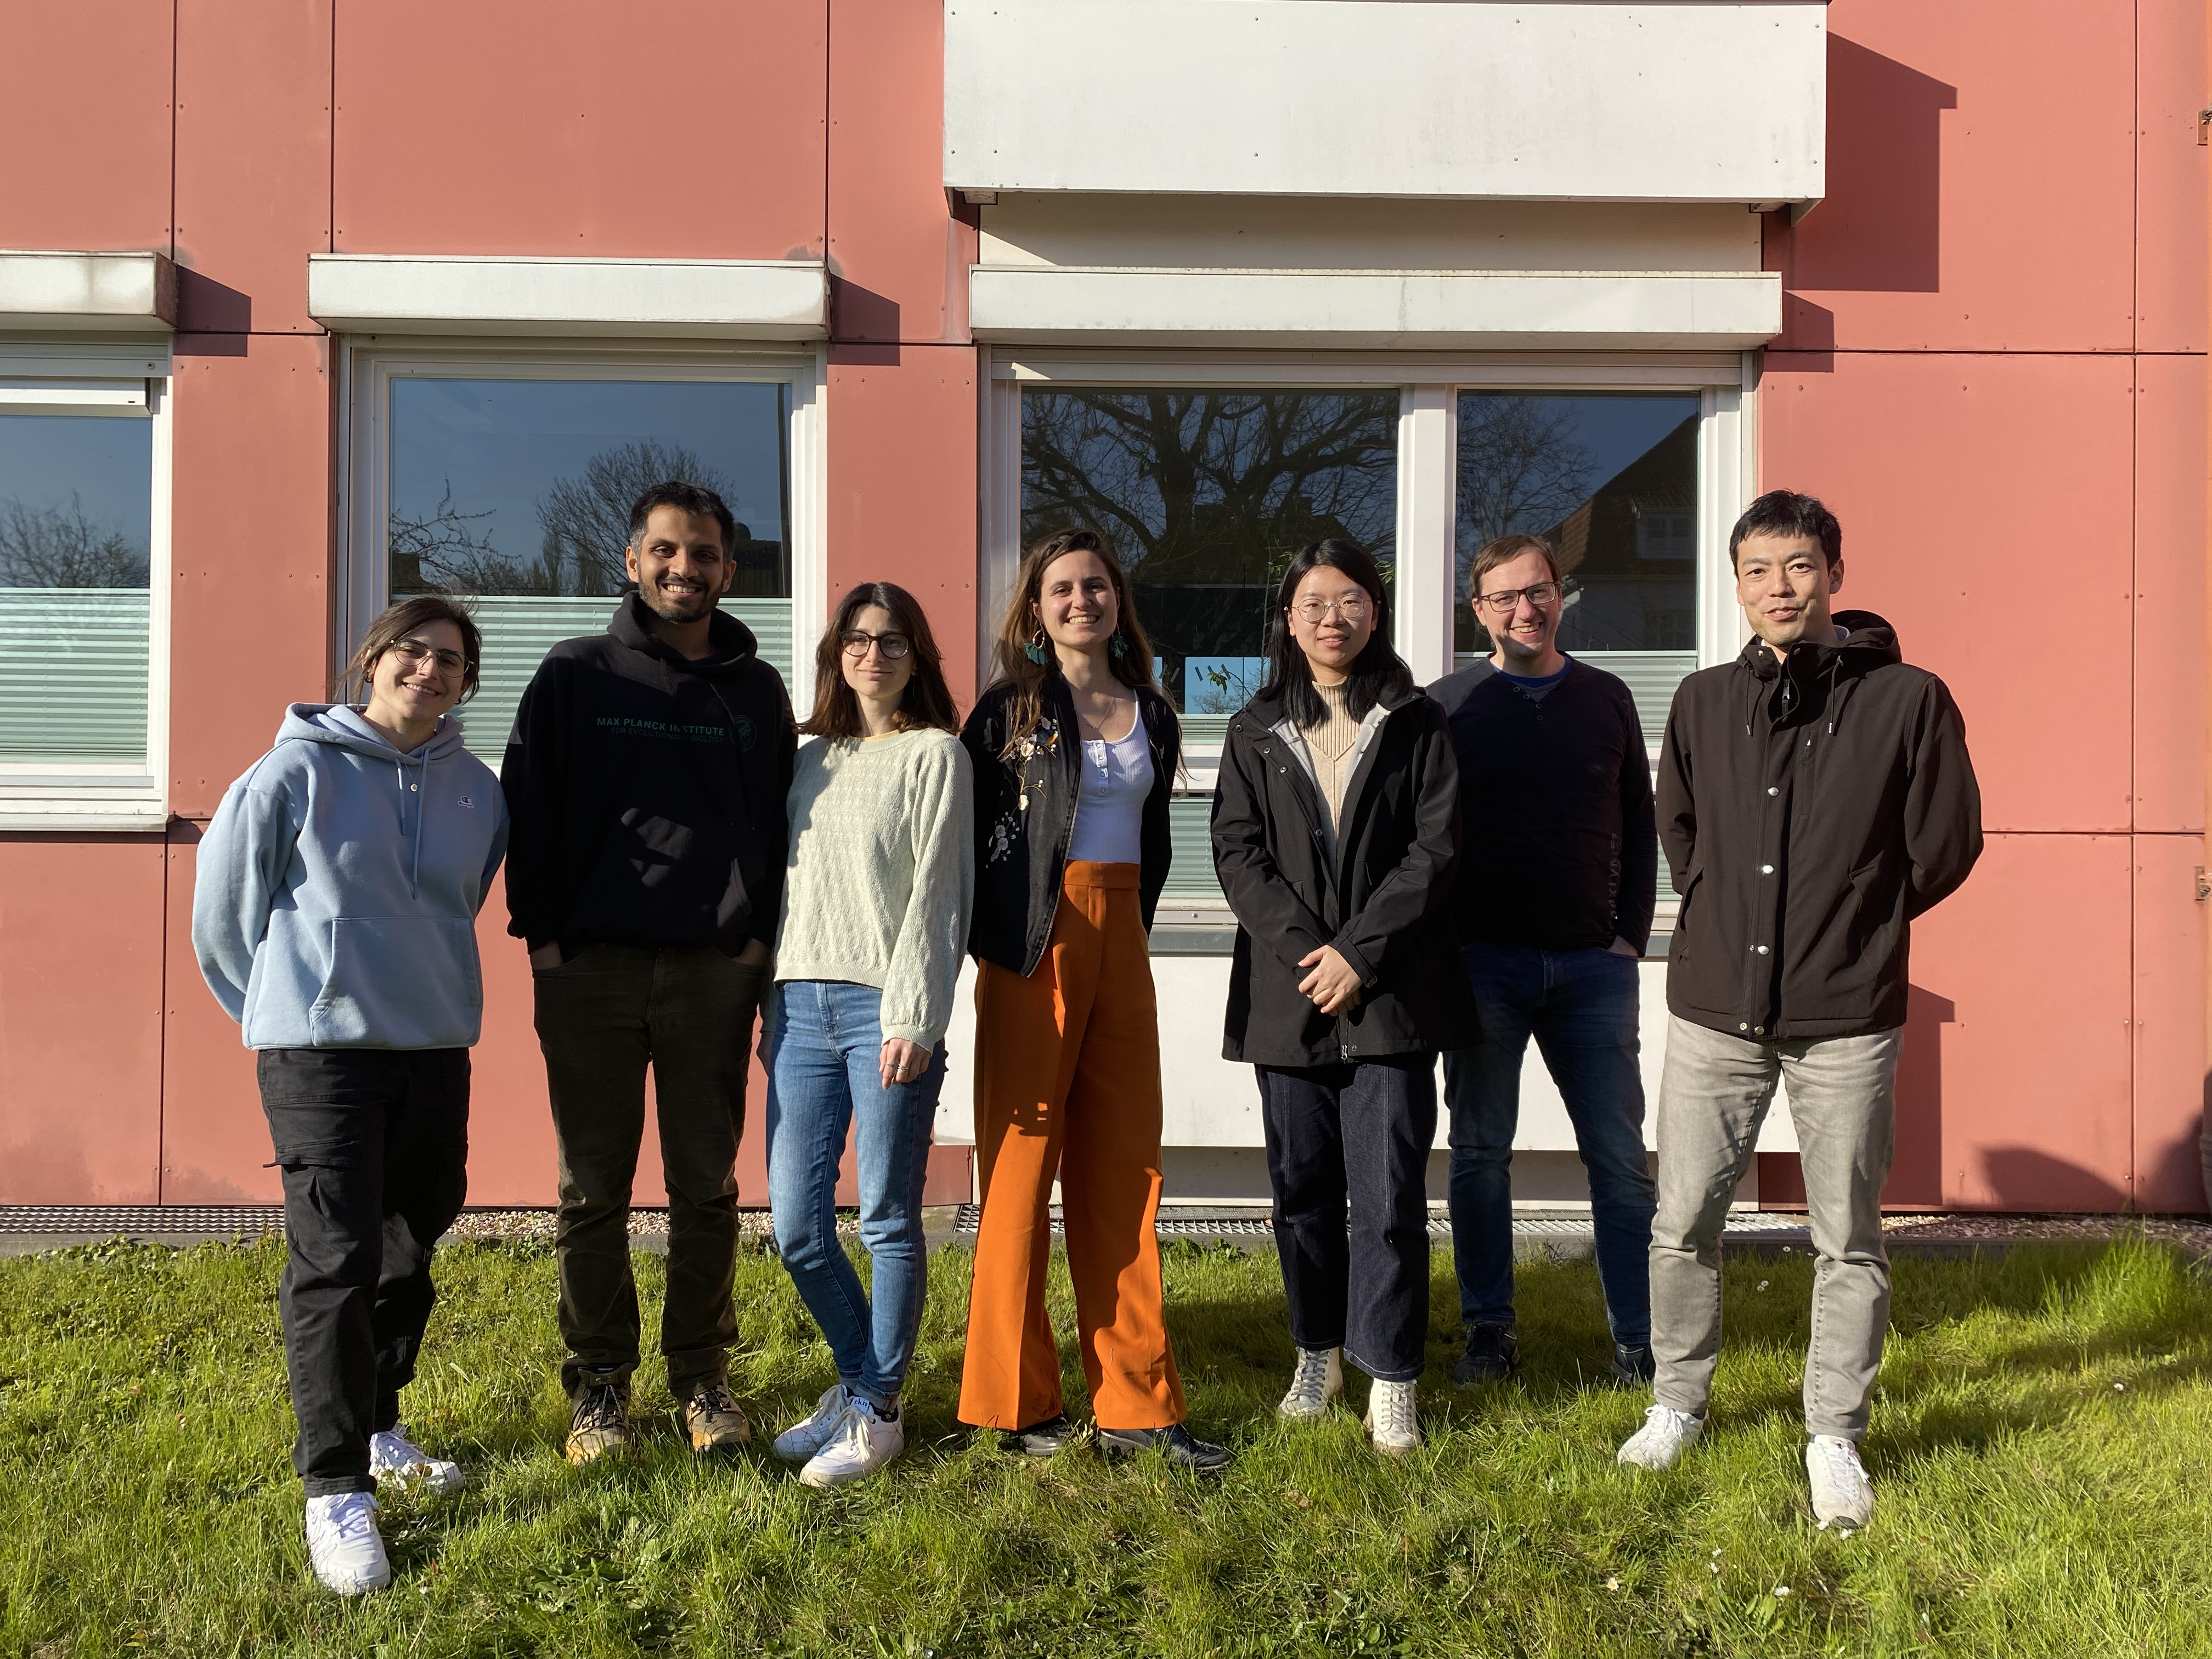
\includegraphics[width=\textwidth]{static/group.jpg}
    \end{column}
    \begin{column}{.4\textwidth}
        \begin{itemize}
            \item Martin Nowak
            \item Ethan Akin
        \end{itemize}
    \end{column}
    \end{columns}
    \end{center}
\end{frame}

\end{document}